\documentclass[a4paper]{article}

\usepackage[utf8]{inputenc}
\usepackage[portuges]{babel}
\usepackage{indentfirst}
\usepackage{graphicx}
\usepackage{float}
\usepackage{caption}
\usepackage{subcaption}
\usepackage[T1]{fontenc}
\usepackage{listings}
\usepackage{amsmath}
\usepackage{mathtools}
\renewcommand{\familydefault}{\sfdefault}

\title{Projeto de Computação Gráfica - Fase 1}
\author{Diogo Braga A82547 \and João Silva A82005 \and Ricardo Caçador A81064
\and Ricardo Veloso A81919}
\date{\today}

\begin{document}

\maketitle

\begin{abstract}
Neste relatório é apresentada a primeira fase dum projeto no qual a intenção é desenvolver um mecanismo baseado em gráficos 3D e fornecer exemplos de uso que mostrem o seu potencial. Este projeto é desenvolvido no âmbito da unidade curricular de Computação Gráfica.
\end{abstract}

\tableofcontents

\newpage


\section{Introdução}
\label{sec:intro}

Esta primeira fase tem como objetivo a criação de duas aplicacões: \textit{generator} e \textit{engine}.

O \textit{generator} cria/reescreve um ficheiro (passado como parâmetro) que contém todos os vértices necessários para o desenho de uma determinada superfície, bem como o número de triângulos no início desse mesmo ficheiro.

No caso do \textit{engine} é necessário que este leia um ficheiro do tipo XML onde se encontra a referência para o ficheiro criado/reescrito, que queremos ler para depois ser gerada a figura pretendida.

De seguida, iremos apresentar todos os algoritmos e equações, bem como as suas respetivas explicações, que foram utilizados para a realização das duas aplicações. Também serão apresentadas figuras que contém código e figuras ilustrativas dos algoritmos/equações.

\section{Estrutura da Pasta do Projeto}
\label{sec:estrutura}

Para um entendimento mais claro da estrutura do projeto, achamos por bem referenciar a estrutura da pasta do projeto.
O projeto entregue contêm para além do relatório, 4 pastas como é possível verificar na seguinte figura.

\begin{figure}[H]
\centering
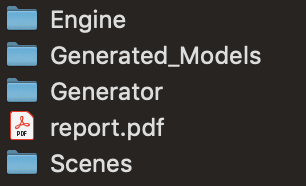
\includegraphics[scale=1.0]{estrutura.png}
\caption{Estrutura da pasta.}
\label{img:estrutura}
\end{figure}

Na pasta \textbf{Engine} residem os ficheiros relativos ao programa \emph{engine}, bem como ficheiros relativos à biblioteca \emph{tinyxml2}. Contém ainda um ficheiro de configuração \emph{cmake}.

Na pasta \textbf{Generator} residem os ficheiros relativos ao programa \emph{generator}. Contém ainda um ficheiro de configuração \emph{cmake}.

Na pasta \textbf{Generated\_Models} residem os ficheiros que contêm os pontos gerados para cada figura, criados pelo programa \emph{generator}.

Na pasta \textbf{Scenes} reside o ficheiro \emph{XML} que contém os nomes dos ficheiros que o programa \emph{engine} tem que carregar posteriormente.


\newpage

\section{Generator}
\label{sec:generator}

\subsection{Explicação dos ficheiros criados}
\label{sec:ficheiros}

Cada função recebe como último parâmetro uma string com o nome do ficheiro que vai guardar os pontos que constituem os triângulos necessários para a criação de cada figura, bem como o número total de triângulos presentes no modelo.

Sendo assim, a primeira linha contém o número de triângulos e todas as linhas seguintes correspondem a um ponto (com as três coordenadas x,y,z separados por um espaço). A junção de três linhas corresponde a um triângulo isto porque um triângulo é definido através de três pontos.

Este processo é feito pelo \textit{generator.cpp} que após ser compilado cria um executável (\textit{Generator}) que terá como argumentos a figura pretendida, os componentes necessários para execução da figura pretendida (por exemplo o raio, as \textit{slices} e as \textit{stacks} no caso da esfera) e o nome do ficheiro a ser criado. Se o ficheiro já existir é reescrito com os novos dados.


\newpage

\subsection{\textit{Plane}}
\label{sec:plane}
A função \textit{generatePlane} recebe como parâmetro um float que representa o comprimento de cada lado do plano (side).

Com base no valor do lado, são gerados os quatro pontos que formam os vértices do plano. Com estes quatros pontos é possível construir os dois triângulos que constituem o quadrado.

\subsubsection{Algoritmo:}

\ttfamily
\begin{enumerate}
  \item Atribuir à variavel parcial\_side o valor de side/2
  \item Construir o primeiro triângulo com os pontos:

        \hspace{2cm} P1 $\Rightarrow$ (parcial\_side, 0.0, -parcial\_side)

        \hspace{2cm} P2 $\Rightarrow$ (-parcial\_side, 0.0, -parcial\_side)

        \hspace{2cm} P3 $\Rightarrow$ (-parcial\_side, 0.0, parcial\_side)
  \item Construir o segundo triângulo com os pontos:

        \hspace{2cm} P1 $\Rightarrow$ (parcial\_side, 0.0, -parcial\_side)

        \hspace{2cm} P3 $\Rightarrow$ (-parcial\_side, 0.0, parcial\_side)

        \hspace{2cm} P4 $\Rightarrow$ (parcial\_side, 0.0, parcial\_side)
  \item Fim
\end{enumerate}
\rmfamily

\begin{figure}[H]
\centering
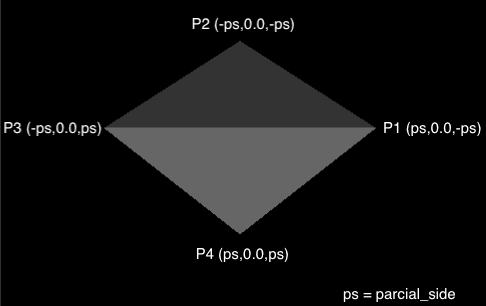
\includegraphics[scale=0.50]{plane.png}
\caption{Vértices do plano}
\label{img:glulookat}
\end{figure}

\newpage

\subsection{\textit{Box}}
\label{sec:box}
A função \textit{generateBox} recebe como parâmetro três floats que representam as dimensões de cada eixo da caixa (X, Y e Z), e um inteiro que representa o número de divisões horizontais (paralelas ao plano xOz) e verticais (paralelas ao plano xOy).

De seguida apresentamos uma imagem de um cubo gerado pela nossa aplicação e a sua explicação através do algoritmo criado pelo grupo.

\begin{figure}[H]
\centering
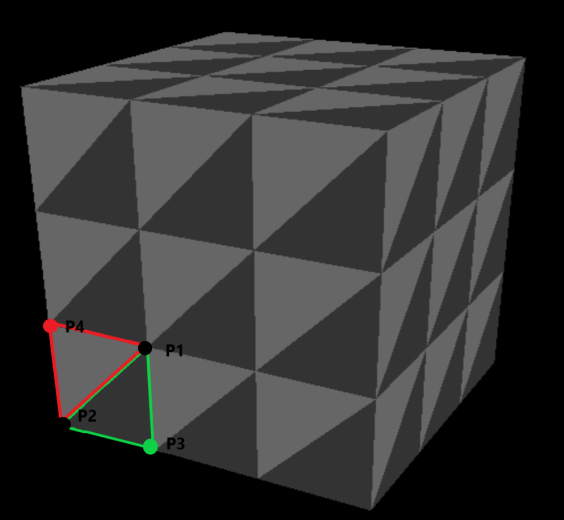
\includegraphics[scale=0.55]{box.png}
\caption{Vértices duma secção da face frontal do plano xOy}
\label{img:Box}
\end{figure}

  \vspace{0.2cm}

\subsubsection{Algoritmo:}

\ttfamily
\begin{enumerate}
  \item Calcular o lado de cada triângulo das divisões, para a dimensão:

  \vspace{0.2cm}

  \hspace{5.0cm}X $\Rightarrow$ \underline{$tam_{x}$}

  \hspace{5.0cm}Y $\Rightarrow$ \underline{$tam_{y}$}

  \hspace{5.0cm}Z $\Rightarrow$ \underline{$tam_{z}$}

  \item Para as faces paralelas ao plano xOy, iterar no eixo y sobre o número de divisões:
  \begin{enumerate}
    \item Estabelecer o valor inicial da coordenada x $\Rightarrow$ $\frac{-xdim}{2}$, de modo a centrar a \textit{box} na origem.
    \item Iterar no eixo x sobre o número de divisões:
    \begin{enumerate}
    \item Construir os quatro triângulos que formam as duas secções (uma na face positiva e outra na face negativa):

      \vspace{0.5cm}

      \underline{Primeiro triângulo:} (face frontal)

      \vspace{0.5cm}

          \hspace{0.5cm} P1 $\Rightarrow$ (x + $tam_{x}$, (i+1) $\times$ $tam_{y}$, z)

      \vspace{0.2cm}

          \hspace{0.5cm} P2 $\Rightarrow$ (x, i $\times$ $tam_{y}$, z)

      \vspace{0.2cm}

          \hspace{0.5cm} P3 $\Rightarrow$ (x + $tam_{x}$, i $\times$ $tam_{y}$, z)

      \vspace{0.5cm}

      \underline{Segundo triângulo:} (face frontal)

      \vspace{0.5cm}

          \hspace{0.5cm} P1 $\Rightarrow$ (x, (i+1) $\times$ $tam_{y}$, z)

      \vspace{0.2cm}

          \hspace{0.5cm} P2 $\Rightarrow$ (x, i $\times$ $tam_{y}$, z)

      \vspace{0.2cm}

          \hspace{0.5cm} P3 $\Rightarrow$ (x + $tam_{x}$, (i+1) $\times$ $tam_{y}$, z)

      \vspace{0.5cm}

      \underline{Terceiro triângulo:} (face traseira)

      \vspace{0.5cm}

          \hspace{0.5cm} P1 $\Rightarrow$ (x + $tam_{x}$, (i+1) $\times$ $tam_{y}$, -z)

      \vspace{0.2cm}

          \hspace{0.5cm} P2 $\Rightarrow$ (x + $tam_{x}$, i $\times$ $tam_{y}$, -z)

      \vspace{0.2cm}

          \hspace{0.5cm} P3 $\Rightarrow$ (x, i $\times$ $tam_{y}$, -z)

      \vspace{0.5cm}

      \underline{Quarto triângulo:} (face traseira)

      \vspace{0.5cm}

          \hspace{0.5cm} P1 $\Rightarrow$ (x, (i+1) $\times$ $tam_{y}$, -z)

      \vspace{0.2cm}

          \hspace{0.5cm} P2 $\Rightarrow$ (x + $tam_{x}$, (i+1) $\times$ $tam_{y}$, -z)

      \vspace{0.2cm}

          \hspace{0.5cm} P3 $\Rightarrow$ (x, i $\times$ $tam_{y}$, -z)

      \vspace{0.5cm}

      \item Somar o valor $tam_{x}$ à variável x.

      \end{enumerate}

    \end{enumerate}

    \item Realizar um ciclo do género para as faces paralelas ao plano zOy.
    \item Realizar um ciclo do género para as faces paralelas ao plano zOx.

    \item Fim
\end{enumerate}
\rmfamily

\newpage

\subsection{\textit{Sphere}}
\label{sec:sphere}

Para calcular os pontos necessários para o desenho da esfera, utilizamos o o raio, o número de slices e o números de stacks. Para calcular coordenadas utilizamos coordenadas esféricas.

Para o cálculo das várias stacks usamos um ângulo $\beta$ que varia entre 0 e $\pi$ com o eixo do Y. Considerando o ângulo $\beta$ desta forma (figura \ref{img:sphere_angles}), podemos resolver todo o algoritmo apenas com um ciclo \emph{for} aninhado. O ângulo de stack em stack avança: $$StackStep = \frac{\pi}{numero\_stacks}\ rads$$

Para o cálculo das várias slices usamos um ângulo $\alpha$ que varia entre 0 e $2\times\pi$ com o eixo do X. O ângulo de slice em slice avança: $$ SliceStep = \frac{2\times\pi}{numero\_slices}\ rads$$

Na seguinte figura é possível analisar o descrito.

\begin{figure}[H]
\centering
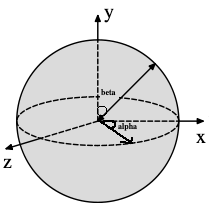
\includegraphics[scale=1.2]{sphere_angles.png}
\caption{Ângulos considerados para a geração de pontos da esfera.}
\label{img:sphere_angles}
\end{figure}

\subsubsection{Algoritmo:}

\ttfamily
\begin{enumerate}
  \item Iterar sobre o número de stacks:
  \begin{enumerate}
    \item Calcular o ângulo $\beta$ para a stack atual $\Rightarrow$ \underline{$\beta_{atual}$}
    \item Calcular o ângulo $\beta$ para a stack seguinte $\Rightarrow$ \underline{$\beta_{seguinte}$}
    \item Calcular o raio da stack atual $\Rightarrow$ \underline{rs} (radius stack)
    \item Calcular o raio da stack seguinte $\Rightarrow$ \underline{rsn} (radius stack next)

    \item Iterar sobre o número de slices:
    \begin{enumerate}
      \item Calcular o ângulo $\alpha$ para o slice atual $\Rightarrow$ \underline{$\alpha_{atual}$}
      \item Calcular o ângulo $\alpha$ para o slice seguinte $\Rightarrow$ \underline{$\alpha_{seguinte}$}
      \item Construir os dois triângulos da stack atual:

      \vspace{0.5cm}

      \underline{Primeiro triângulo:}

      \vspace{0.5cm}

          \hspace{0.0cm} P1 $\Rightarrow$ (rs $\times$ cos($\alpha_{atual}$) , r $\times$ cos($\beta_{atual}$), rs $\times$ cos($\alpha_{atual}$))

      \vspace{0.2cm}

          \hspace{-0.5cm} P2 $\Rightarrow$ (rsn $\times$ cos($\alpha_{seguinte}$) , r $\times$ cos($\beta_{seguinte}$), rsn $\times$ sin($\alpha_{seguinte}$))

      \vspace{0.2cm}

          \hspace{0.0cm} P3 $\Rightarrow$ (rsn $\times$ cos($\alpha_{atual}$) , r $\times$ cos($\beta_{seguinte}$), rsn $\times$ sin($\alpha_{atual}$))

      \vspace{0.5cm}

      \underline{Segundo triângulo:}

      \vspace{0.5cm}

          \hspace{-0.25cm} P1 $\Rightarrow$ (rs $\times$ cos($\alpha_{seguinte}$) , r $\times$ cos($\beta_{atual}$), rs $\times$ sin($\alpha_{seguinte}$))

      \vspace{0.2cm}

          \hspace{-0.75cm} P2 $\Rightarrow$ (rsn $\times$ cos($\alpha_{seguinte}$) , r $\times$ cos($\beta_{seguinte}$), rsn $\times$ sin($\alpha_{seguinte}$))

      \vspace{0.2cm}

          \hspace{0.0cm} P3 $\Rightarrow$ (rs $\times$ cos($\alpha_{atual}$) , r $\times$ cos($\beta_{seguinte}$), rs $\times$ sin($\alpha_{atual}$))

      \vspace{0.2cm}

    \end{enumerate}

    \end{enumerate}

    \item Fim
    \end{enumerate}
    \rmfamily

\begin{figure}[H]
\centering
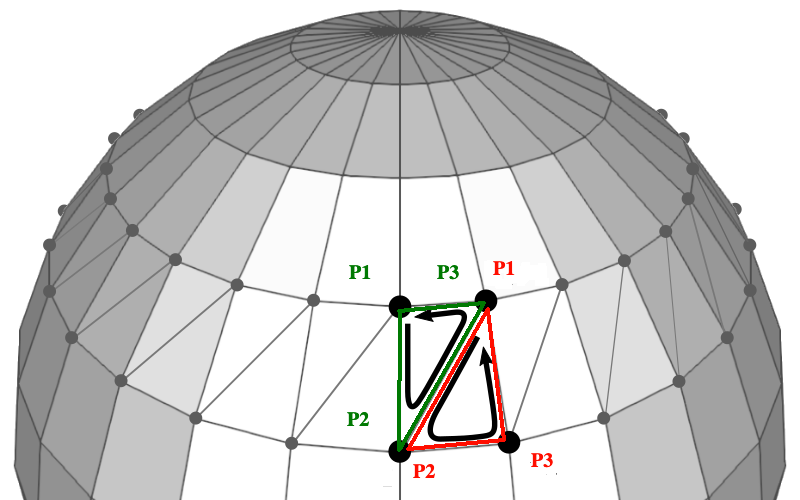
\includegraphics[scale=0.50]{stacks_sphere.png}
\caption{Cálculo dos 2 triângulos duma dada stack.}
\label{img:stack_sphere}
\end{figure}

Ao percorrer todas as slices em cada iteração do algoritmo, desenha-se cada quadrilátero recorrendo a dois triângulos como descrito no algoritmo acima. Na figura \ref{img:stack_sphere} o triângulo a vermelho corresponde ao primeiro triângulo que é calculado, consequentemente, o triângulo a verde é o segundo a ser calculado.

\newpage

\subsection{\textit{Cone}}
\label{sec:cone}
A função \textit{generateCone} recebe como parâmetro um float que representa o raio da base do cone, um float que representa a altura do cone, um inteiro que representa o número de triângulos que queremos que constituam a base, e ainda outro inteiro que representa o número de \textit{stacks} que constituem o lado do cone.


\begin{figure}[H]
\centering
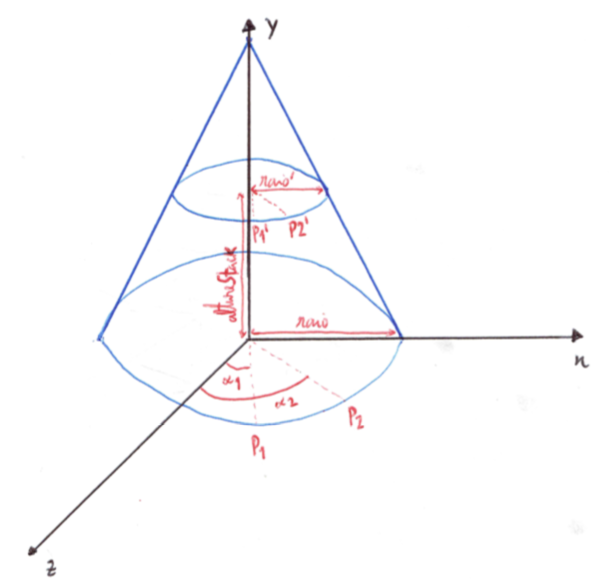
\includegraphics[scale=0.50]{cone_pontos.png}
\caption{Calcular as coordenadas de um ponto na superfície do cone}
\label{img:cone_pontos}
\end{figure}

\ttfamily
$$\alpha_{1} = slice\_atual \times \frac{2\pi}{numero\_slices} $$

\vspace{0.5cm}

$$\alpha_{2} = (slice\_atual+1) \times \frac{2\pi}{numero\_slices} $$

\vspace{0.5cm}

        \hspace{1.5cm} P1 $\Rightarrow$ (raio $\times$ cos($\alpha_{1}$) , 0.0, raio $\times$ sin($\alpha_{1}$))

\vspace{0.2cm}

        \hspace{1.5cm} P2 $\Rightarrow$ (raio $\times$ cos($\alpha_{2}$) , 0.0, raio $\times$ sin($\alpha_{2}$))

\vspace{0.2cm}

        \hspace{0.5cm} P1' $\Rightarrow$ (raio' $\times$ cos($\alpha_{1}$) , altura\_stack, raio' $\times$ sin($\alpha_{1}$))

\vspace{0.2cm}

        \hspace{0.5cm} P2' $\Rightarrow$ (raio' $\times$ cos($\alpha_{2}$) , altura\_stack, raio' $\times$ sin($\alpha_{2}$))

\rmfamily

\vspace{1cm}

\begin{figure}[H]
\centering
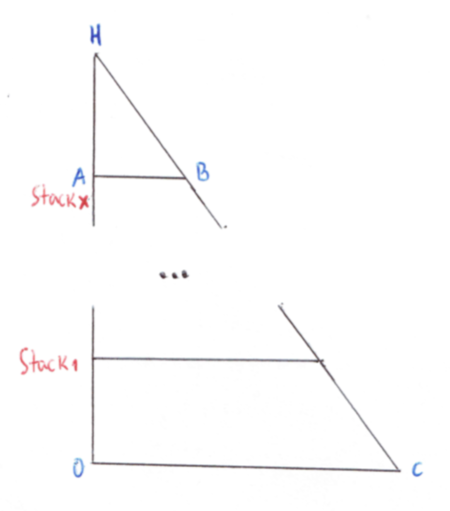
\includegraphics[scale=0.50]{cone_raio_altura.png}
\caption{Calcular o raio e a altura de uma stack}
\label{img:cone_raio_altura}
\end{figure}

\ttfamily

Pela Regra dos Triângulos Semelhantes:

$$ \frac{HA}{HO} = \frac{AB}{OC} \Leftrightarrow $$

\vspace{0.5cm}

$$ \Leftrightarrow \frac{altura - altura\_stack}{altura} = \frac{raio\_stack}{raio} \Leftrightarrow $$

\vspace{0.5cm}

$$ \Leftrightarrow raio\_stack = \frac{(altura - altura\_stack) \times raio}{altura} $$

\vspace{1cm}

$$ altura\_stack = \frac{altura}{stacks} \times numero\_stack $$

\newpage

\subsubsection{Algoritmo:}

\ttfamily
\begin{enumerate}
  \item Iterar sobre o número de slides:
  \begin{enumerate}
    \item Calcular o ângulo $\alpha$ para o slice atual $\Rightarrow$ \underline{$\alpha_{atual}$}
    \item Calcular o ângulo $\alpha$ para o slice seguinte $\Rightarrow$ \underline{$\alpha_{seguinte}$}
    \item Construir os pontos do triângulo formado pelas duas slices atuais:

    \vspace{0.2cm}

        \hspace{3cm} P1 $\Rightarrow$ (0.0, 0.0, 0.0)

    \vspace{0.2cm}

        \hspace{1cm} P2 $\Rightarrow$ (raio $\times$ cos($\alpha_{atual}$) , 0.0, raio $\times$ sin($\alpha_{atual}$))

    \vspace{0.2cm}

        \hspace{0.5cm} P3 $\Rightarrow$ (raio $\times$ cos($\alpha_{seguinte}$) , 0.0, raio $\times$ sin($\alpha_{seguinte}$))

    \vspace{0.3cm}

    \item Guardar altura atual para usar na seguinte iteração $\Rightarrow$ \underline{ph} (previous height)
    \item Guardar raio atual para usar na seguinte iteração $\Rightarrow$ \underline{pr} (previous radius)

    \item Iterar sobre o número de stacks, exceto a última:
    \begin{enumerate}
      \item Calcular a altura da stack atual $\Rightarrow$ \underline{nh} (new height)
      \item Calcular o raio da stack atual $\Rightarrow$ \underline{nr} (new radius)
      \item Construir os dois triângulos da stack:

      \vspace{0.5cm}

      \underline{Primeiro triângulo:}

      \vspace{0.5cm}

          \hspace{0.5cm} P1 $\Rightarrow$ (nr $\times$ cos($\alpha_{atual}$) , nh, nr $\times$ sin($\alpha_{atual}$))

      \vspace{0.2cm}

          \hspace{0.25cm} P2 $\Rightarrow$ (pr $\times$ cos($\alpha_{seguinte}$) , ph, pr $\times$ sin($\alpha_{seguinte}$))

      \vspace{0.2cm}

          \hspace{0.5cm} P3 $\Rightarrow$ (pr $\times$ cos($\alpha_{atual}$) , ph, pr $\times$ sin($\alpha_{atual}$))

      \vspace{0.5cm}

      \underline{Segundo triângulo:}

      \vspace{0.5cm}

          \hspace{0.5cm} P1 $\Rightarrow$ (nr $\times$ cos($\alpha_{atual}$) , nh, nr $\times$ sin($\alpha_{atual}$))

      \vspace{0.2cm}

          \hspace{0.25cm} P2 $\Rightarrow$ (nr $\times$ cos($\alpha_{seguinte}$) , nh, nr $\times$ sin($\alpha_{seguinte}$))

      \vspace{0.2cm}

          \hspace{0.25cm} P3 $\Rightarrow$ (pr $\times$ cos($\alpha_{seguinte}$) , ph, pr $\times$ sin($\alpha_{seguinte}$))

      \vspace{0.2cm}
      \item Guardar a altura e raio desta stack
    \end{enumerate}

    \vspace{0.2cm}

    \item Construir o triângulo da ponta do cone (última stack), formado pelos pontos:

    \vspace{0.5cm}

        \hspace{3cm} P1 $\Rightarrow$ (0.0, height, 0.0)

    \vspace{0.2cm}

        \hspace{0.5cm} P2 $\Rightarrow$ (pr $\times$ cos($\alpha_{seguinte}$) , ph, pr $\times$ sin($\alpha_{seguinte}$))

    \vspace{0.2cm}

        \hspace{1cm} P3 $\Rightarrow$ (pr $\times$ cos($\alpha_{atual}$) , ph, pr $\times$ sin($\alpha_{atual}$))

    \vspace{0.3cm}

  \end{enumerate}

  \item Fim
\end{enumerate}
\rmfamily

\begin{figure}[H]
\centering
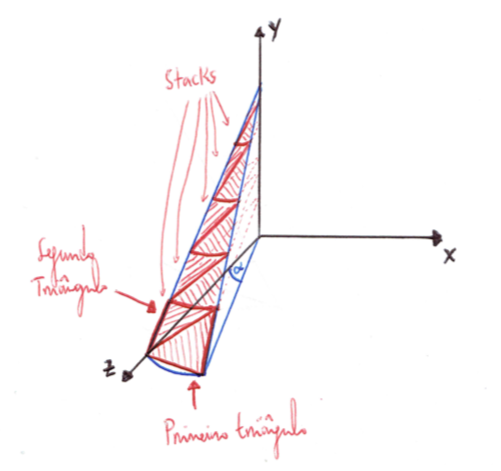
\includegraphics[scale=0.50]{cone_triangulos.png}
\caption{Triângulos das stacks}
\label{img:cone_triangulos}
\end{figure}

\newpage

\section{Engine}
\label{sec:engine}
De forma a representar as figuras de uma determinada cena, usou-se XML para referenciar os ficheiros construídos pelo \emph{generator}. Esses ficheiros contêm vários pontos que dão resultado a vários triângulos, que resultam em figuras.

No caso de exitir mais do que um modelo a ser carregado, as figuras encontrar-se-ão sobrepostas aquando o seu desenho no ecrã.

\begin{figure}[H]
\centering
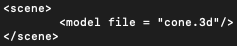
\includegraphics[scale=0.70]{scene_xml.png}
\caption{Exemplo "scene.xml"}
\label{img:scene}
\end{figure}

Na aplicação criada, foram criadas duas classes:

\hspace{1cm} \texttt{Point}

\hspace{1cm} Contém três \texttt{float (x,y,z)} que representam as coordenadas do ponto.

\hspace{1cm} \texttt{Figure}

\hspace{1cm} Contém o número de triângulos e um \texttt{vector} com vários \texttt{Point}.

\subsection{Ficheiro XML}
Para o parsing do documento XML utilizamos a API do tinyXML2.

A função \texttt{load\_generated\_files()} é responsável pela leitura do ficheiro XML e gravar os pontos lidos em memória para que depois sejam utilizados para a criação das figuras.

O algoritmo para esta função é descrito de seguida.

\begin{enumerate}
	\item Abre o ficheiro "scene.xml" (em caso de erro, termina execução e envia mensagem de erro);
	\item Procura primeiro elemento "scene" e em caso de erro, termina a execução;
	\item Cria um vetor onde serão armazenadas as figuras que queremos carregar para posteriormente desenhar - \texttt{vector<string> files};
	\item Itera sobre todas as linhas com o elemento model:

	\begin{enumerate}
		\item Cria uma string "new\_file" que contém o nome da figura a carregar
		\item Insere a string "new\_file" no vetor \texttt{files}
	\end{enumerate}

	\item Itera sobre o vetor files:

	\begin{enumerate}
		\item Abre o ficheiro correspondente ao nome da string;
		\item Cria uma \texttt{Figure} fig:

		\begin{enumerate}
			\item Lê o numero de triângulos do ficheiro e guarda em fig.
			\item Até ao final do ficheiro cria um \texttt{Point} new\_point onde irá ser gravado os componentes x,y e z e coloca este em fig.
		\end{enumerate}
		\item Coloca fig em figures que é a estrutura utilizada para gravar as figuras a desenhar.
	\end{enumerate}
\end{enumerate}

Todo este processo resulta na presença de todas as figuras a desenhar, estarem em memória.

\subsection{Desenho das figuras}

Após a realização do processo anterior, vamos proceder ao desenho das figuras gravadas em memória. Para tal desenvolvemos uma função \textbf{load\_figures()} cujo o algoritmo é apresentado de seguida.

\begin{enumerate}
	\item Iteramos sobre o vetor figures:
	 \begin{enumerate}
	 	\item Guarda no vetor \texttt{current\_point} os pontos da figura a desenhar.
	 	\item Inicia o desenho da figura (através da função \texttt{glBegin(GL\_TRIANGLES)});
	 	\item Iteramos sobre o vetor \texttt{current\_point}:
	 	\begin{enumerate}
	 		\item Definimos que a cada três pontos a cor é alterada (ou seja, por triângulo).
	 		\item Representa o ponto utilizando a função \texttt{glVertex3f} dando como argumentos as componentes x,y e z do \texttt{current\_point};
	 	\end{enumerate}
	 	\item Terminar o desenho da figura com \texttt{glEnd()}.
	 \end{enumerate}
\end{enumerate}

\section{Câmera}
\label{sec:camera}
De forma a poder visualizar as figuras de diferentes ângulos criamos uma câmera que pode variar a sua posição e o ponto para que está a olhar, mantendo-se portanto todas as figuras geradas fixas.

Por forma a mover a posição da câmera usamos as teclas UP, DOWN, LEFT e RIGHT. Desta forma a câmera altera a sua posição consoante um ângulo $\alpha$ que varia no plano XZ, e um ângulo $\beta$ que varia no plano XY. Inicialmente é ainda definido um raio, que em conjunto com os ângulos falados faz com que a câmera varie a sua posição como se estivesse assente numa superfície esférica. Este raio pode ainda ser mudado por forma a aproximar ou afastar a câmera do ponto para o qual está a olhar. Tal é feito através das teclas '+' e '-'.

É também possível alterar o ponto para o qual a câmera está a olhar. Esta ação pode ser feita através das teclas A,S,D,Q,W e E que alteram as coordenadas de X, Y e Z do ponto para o qual a câmera deve olhar.

Por forma ainda de visualizar as figuras de diferentes modos utilizamos as teclas Z, X e C, que alteram a forma de visualização para linhas, pontos, e preenchido.

\begin{figure}[H]
\centering
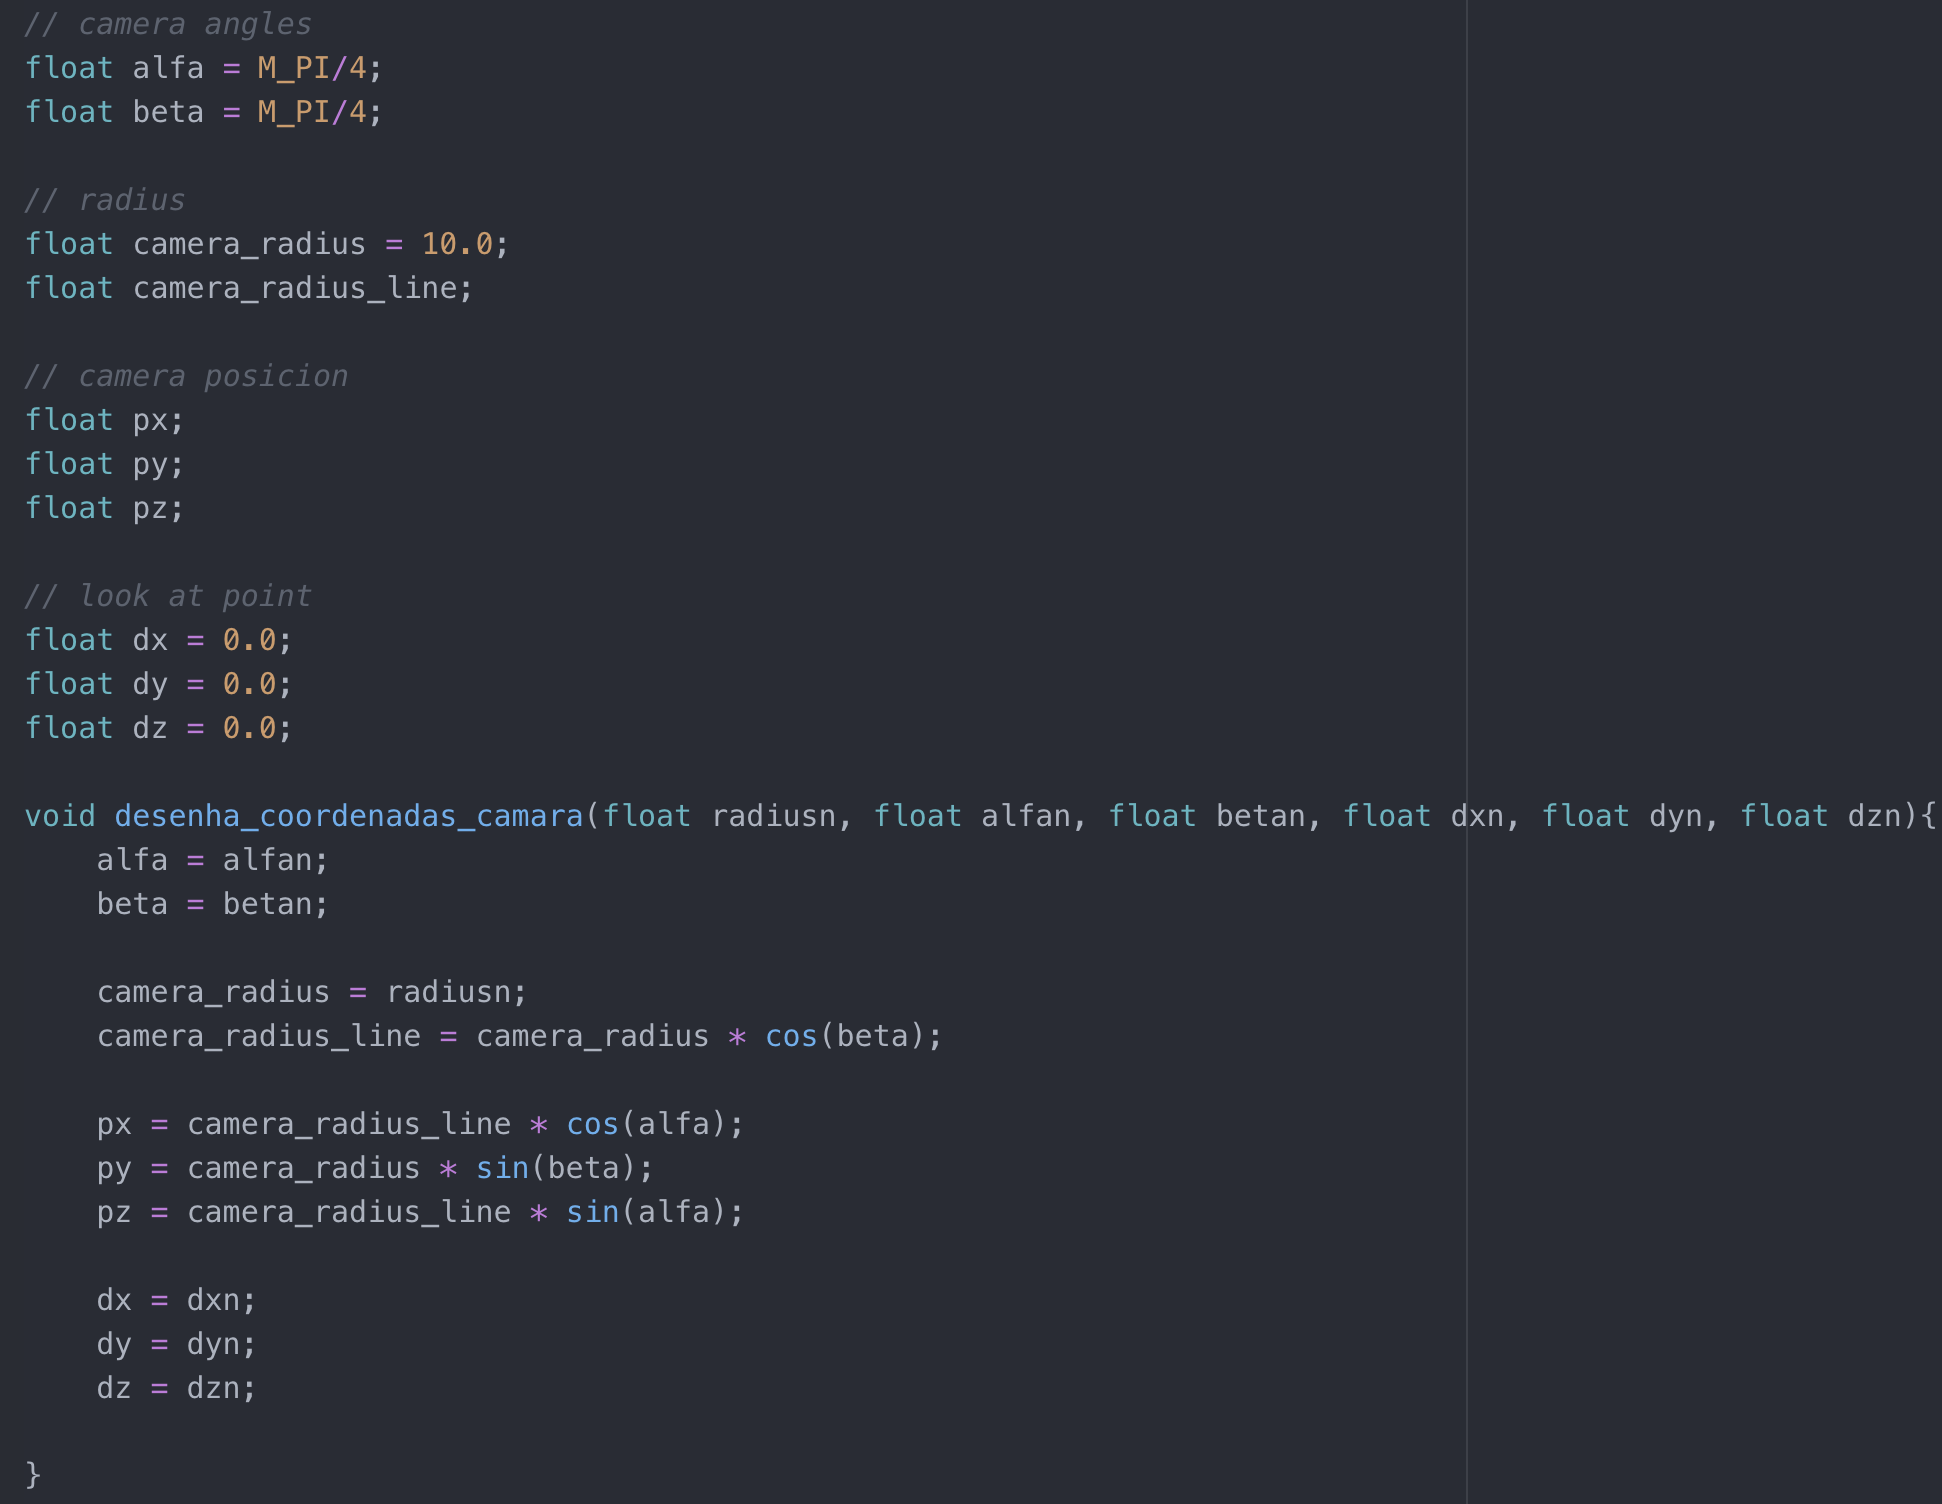
\includegraphics[scale=0.40]{funcao_desenha.png}
\caption{Função encarregue dos parâmetros da câmara.}
\label{img:desenha}
\end{figure}

Como é descrito na figura \ref{img:desenha}, realizamos uma função que está encarregue de atualizar e gerir todos os parâmetros referentes à câmera. Esta função é realizada consoante qualquer alteração num destes parâmetros.

Por forma a envolver diretamente estes parâmetros com a câmera, inserimo-los na função \emph{gluLookAt()}, como é possível visualizar na figura \ref{img:glulookat}.

\begin{figure}[H]
\centering
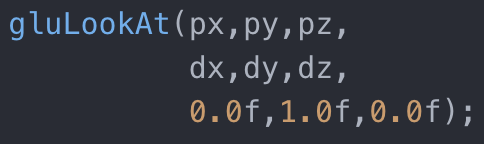
\includegraphics[scale=0.70]{gluLookAt.png}
\caption{Função que contém a matriz da câmera.}
\label{img:glulookat}
\end{figure}

A câmera é também um mecanismo muito forte de deteção de erros, uma vez que nos permite visualizar as figuras de várias formas e perspetivas.


\section{Conclusão}
\label{sec:conclusao}

Terminada a realização da fase 1 - primitivas gráficas, o grupo sente que realizou com sucesso  as 4 primitivas gráficas que compunham esta fase (plane, box, sphere e cone).  Assim, depois de uma revisão integral ao trabalho achamos que estamos preparados e num bom caminho para a realização de um bom projeto.
No geral não sentimos muitas dificuldades em nenhuma das primitivas gráficas pois também contamos com a ajuda da câmera que implementamos que permitiu uma melhor visualização do que estávamos a fazer bem ou mal.



\end{document}
